%Glossary of components, terms

\section{Glossary}
\label{sec:glossary}
\begin{longtable}{| l | l| l |}
\hline
\textbf{Component} & \textbf{Description} & \textbf{Quantity} \\ \hline
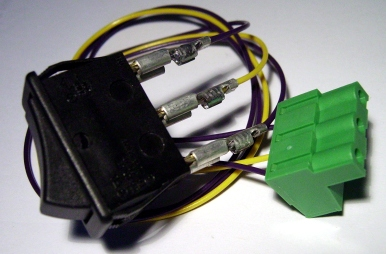
\includegraphics[width=4cm]{chrg-run-sw}  & Charge/Run switch & 1 \\ \hline
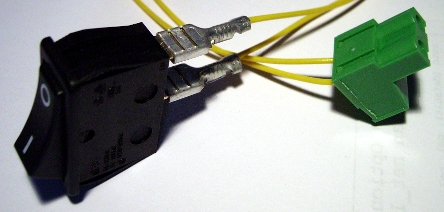
\includegraphics[width=4cm]{on-off-sw}  & On/Off Switch & 1 \\ \hline
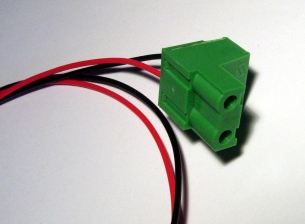
\includegraphics[width=4cm]{battery-con}  & Battery Connector & 1 \\ \hline
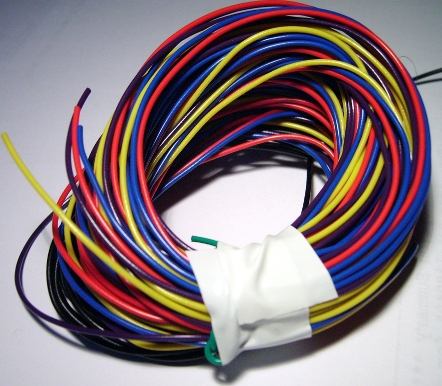
\includegraphics[width=4cm]{wire}  & Multi-core Electrical Wire & 5 \\ \hline
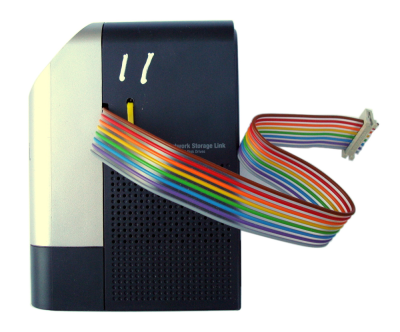
\includegraphics[width=4cm]{slug}  & Slug & 1 \\ \hline
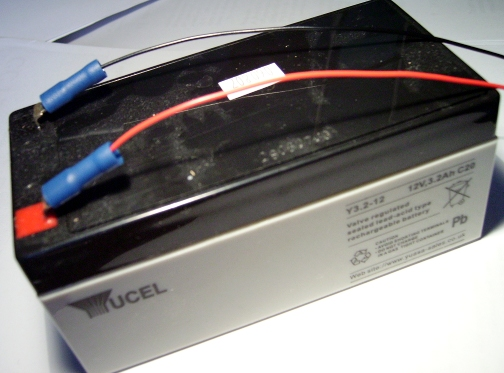
\includegraphics[width=4cm]{battery}  & 12V Sealed Lead Acid battery & 1 \\ \hline
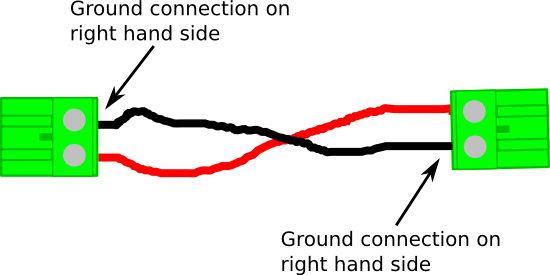
\includegraphics[width=4cm]{camcon}  & SR Connector & 4 \\ \hline
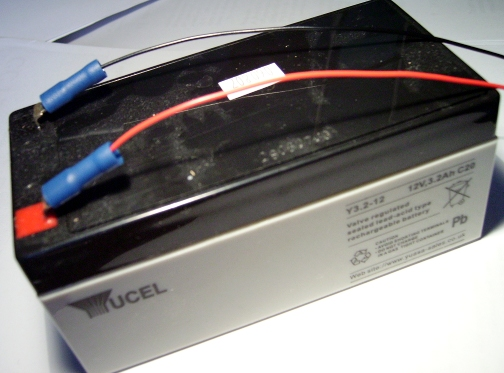
\includegraphics[width=4cm]{battery}  & 12V Sealed Lead Acid battery & 1 \\ \hline
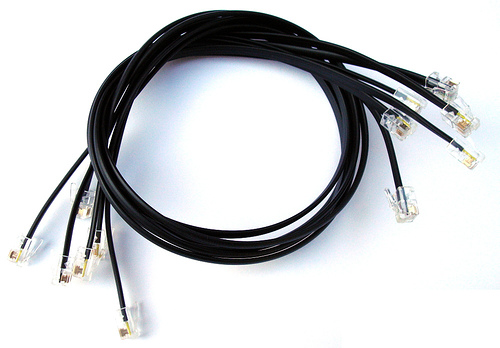
\includegraphics[width=4cm]{4p4c}  & RJ11 Cable & 5 \\ \hline
[photo]  & USB Memory Stick & 2 \\ \hline
[photo]  & Battery Charger & 1 \\ \hline
[photo]  & PCB Spacers & 16 \\ \hline
\end{longtable}
